\section{Scores definition}

In this section, we propose the \gls{ALE}-based scores that allow the computation of 1) a more isolated individual effects of variables 2) to give different insights in the data-generating process even when data is not independent.   Initially, this section presents metrics analogous to the coefficients in linear models, capable of reporting both the magnitude and direction of feature effects. Subsequently, it discusses a metric that only quantifies the overall relevance of features.

Formulating a single score to represent the effect size of a feature presents a complex challenge. In linear models, where the effects of features remain constant across their entire range, the slope obtained from the \gls{ALE} method corresponds exactly with the linear model's coefficients. Utilizing a Bootstrap sampling approach in this scenario could potentially yield a confidence interval closely akin to that obtained through t-statistics, as illustrated in Table \ref{table:linear_regression_ci}. However, this does not hold true for non-linear models. In such cases, assigning a single numerical value to express feature effects often fails to capture their intricate dimensions fully. Instead, a complete \gls{ALE} plot is required to comprehensively capture the nuances of feature effects. 

Nevertheless, considering  \gls{ALE}'s decomposition property (see: Section \ref{centerAle}), scores can meaningfully represent the individual effects of features if explicitly defined. For instance, ALE calculates isolated effects within specific data segments. When these segments are not too narrow or too broad and representative of the wider population, with minimal prediction noise, they can be particularly informative. In such cases, identifying the segment with the most pronounced feature effects can yield valuable insights into the degree to which a feature impacts the target variable. This is especially relevant for considering potential interventions in the current dataset. 

The potential interventions are safeguarded due to \gls{ALE}'s implementation, which performs the do-operator (see: Section \ref{intervention}) for every data point of the segment. For instance, it can be insightful for the educational practitioner to understand that, regardless of individual differences, a potential educational policy (represented by one feature) may not be able to change the chances of any student success (target variable) more than a specified threshold. Similarly, finding out that an underlying policy tends to yield great results for a representative group of students can drive further research to determine who benefits most and who does not. Furthermore, the effect of a feature at a specific value can reveal its individual impact on a particular group of interest of the researcher. 

Building on this thought, four new metrics for feature effect size have been introduced. To ensure more reliable estimations, these metrics are designed to be computed on unseen data, distinct from the data on which the model was trained, as detailed in Algorithm \ref{algorithm:cap3}:

\begin{table}[h]
\centering
\rowcolors{1}{}{lightgray}
\begin{tabular}{|c||c|c|c||c|c|c|}
\hline
Feature & Slope & Lower CI & Upper CI & ALE\_slope & Lower CI & Upper CI \\
\hline
0 &44.018 &44.015 & 44.021 & 44.021 & 44.015 & 44.027 \\
1 &-0.0025 &-0.006 & 0.001 & 0.001 & -0.006 & 0.007 \\
2 &-0.004 &-0.007 & -0.001 & -0.000 & -0.007 & 0.005 \\
3 &73.229 &73.226 & 73.232 & 73.232 & 73.226 & 73.239 \\
4 &52.552 &52.549 & 52.555 & 52.555 & 52.548 & 52.561 \\
5 &9.5595 &9.556 & 9.563 & 9.563 & 9.557 & 9.568 \\
6 &63.286 &63.283 & 63.289 & 63.289 & 63.283 & 63.295 \\
7 &13.519 &13.516 & 13.522 & 13.522 & 13.516 & 13.528 \\
8 &69.562 &69.559 & 69.565 & 69.565 & 69.559 & 69.572 \\
9 &40.185 &40.182 & 40.188 & 40.188 & 40.182 & 40.195 \\
\hline
\end{tabular}

\caption{Demonstration of the similarity of the coefficients and confident intervals of a linear regression and the slope computed from the ALE plot under a bootstrap sampling on artificial data}
\label{table:linear_regression_ci}
\end{table}



\begin{algorithm}
\caption{Estimating ALE-based scores with optional uncertainty estimation}\label{algorithm:cap3}
\begin{algorithmic}[1]
\Require model \( f \), data \( D = \{X_1, X_2, \ldots, X_k\} \), int \( j \) 
\State Optional: Apply a sampling strategy (cross-validation or bootstrap) on \( D \)
    %\State(retrain model \(f\))
\State Compute quantiles \( Q \) of order \( j \) using \( D \) for the target feature \( X_k \), \( q \`in \{1,...,Q^{k}\} \)
\For{\( q \in Q^{k} \)}
    \State \( \hat{X}_{max} := X \) do(\( x_k := \max(q) \))
    \State \( \hat{X}_{min} := X \) do(\( x_k := \min(q) \))
    \State \( LE_{q}(k) := f(\hat{X}_{max}) - f(\hat{X}_{min}) \) 
\EndFor
    \State $ALE(k) = \sum_{q=1}^{Q^{K}} LE_{q}(k)$
    \State Compute score based on a matrix \( ALE(k) \) of size \( j X k \) 
\end{algorithmic}
\end{algorithm}


The ALE function is defined as a summation of local effects ascertained by the partial derivative. However, in practice, \gls{ALE} implementations employ quantiles. The definition of quantiles already presents a challenge for accurately recovering feature effects under the visualization of \gls{ALE} plots and further influences the precision and correctness of scores interpretation. Specifically, small quantiles may model noise, while larger quantiles may fail to uphold the inherent linearity assumptions of \gls{ALE} within quantiles. 

Therefore, for a more reliable interpretation of the scores, the quantiles (as defined by $j$ in Algorithm \ref{algorithm:cap3}, line 2) should be representative of the sample. This representation should be meaningful within the domain context to reveal its summarized feature effects, while assuming linear feature effects within each quantile. In the domain of education, deciles and quantiles are common units of interest \cite{Carnoy2022TrendsBrazil, Carnoy2017IntranationalBrazil}

Lastly, to account for the uncertainty inherent in the model and data, the metrics can be calculated using a cross-validation approach or a bootstrap sampling strategy. While Bootstrap allows for the construction of confidence intervals by the cost of high computational cost, cross-validation can produce generalized estimates with low computational effort. The \gls{ALE} computation is relatively stable in absence of outliers, as the definition of quantiles tends to remain consistent. This stability is especially notable when the unique values of a feature are few or closely to the \(J\) definition. The greatest source of uncertainty typically lies within the model itself, as an algorithm may approximate different functions while delivering comparably effective performance. If outliers are present, appropriate handling would involve winsorizing the data distribution's tails or adjusting the quantile estimation method to minimize the influence of extreme values on predictions


In Line 9, in Algorithm \ref{algorithm:cap3}, the process for summarizing the influence of a feature on model predictions is defined. Within this context, three metrics are first introduced, calibrated to the same scale as the model's output, offering insights into both the magnitude and direction of the feature's effect size. For clarity, these metrics are didactically compared to the traditional coefficients of linear models. Subsequently, a fourth metric, based on a ranking system, is introduced.

Consider:
\( j \) represents the feature of interest
\( k \) the quantile for feature \( j \).
\( ALE_{j(k)} \) represents the uncentered Accumulated Local Effect for a specific feature \( j \) up to the \( k \)-th quantile.
\( {z_1}_{j(k)} \) is the lower bound of the \( k \)-th quantile for feature \( j \).
\( {z_2}_{j(k)} \) is the upper bound of the \( k \)-th quantile for feature \( j \).
\( n \) is a specific value of interest of \( j \) 

\textbf{1) \gls{MUA}}: the \gls{MUA} metric urges actionability and extracts the maximum change in the predictions (\(y\)) that a feature of interest may derive. The maximum is related to a specific data interval and may be positive or negative, requiring a previous absolute comparison to achieve the highest value.


\begin{equation}
\label{eq:MUA}
\text{MUA}(j) = \max_{k} ALE_{j(k)}
\end{equation}


\textbf{2) \gls{UAS}}:
the \gls{UAS} is an arbitrary choice of a specific value \(n\) of the feature of interest. In practice, it requires discovering into which quantile this value falls and returns the accumulated uncentered ALE up this quantile. This metric may be helpful when the analyst has sufficient domain knowledge or is verifying hypotheses.

\begin{equation}
\label{eq:UAS}
\text{UAS}(j, n) = ALE_{j(k)} \, | \, {z_1}_{j(k)} \leq n \leq {z_2}_{j(k)}
\end{equation}

\textbf{3) \gls{AUA}}: the \gls{AUA} represents the first-order moment of the distribution and offers insights into the general magnitude and direction of feature effects across specified intervals. The \gls{AUA} captures the average isolated impact of a feature of interest on the predictions over these intervals. A lower \gls{AUA} value does not necessarily indicate an insignificant variable; rather, it may reflect a variable with a lower average effects. 

\begin{equation}
\label{eq:AUA}
\text{AUA}(j) = \frac{1}{K} \sum_{k=1}^{K} ALE_{j(k)}
\end{equation}


\subsection{An analogy to the coefficients of linear regression}

This section draws a simplified analogy between the coefficients of linear regression and the newly introduced metrics (\gls{MUA}, \gls{AUA}, and \gls{UAS}). This analogy is instrumental as the coefficients represent completely different measures. However, it will be important to demonstrate how the new metrics can support research inquiries in the field of education.

In linear regression, the coefficients of a variable quantify its overall effect size. When a variable's effect is not constant across its distribution, interaction terms are introduced. These terms account for the variable's differential impact across specific segments of its distribution, such as quartiles. Consider the following model:

\begin{equation}
\label{eq:lm+inter+analogy}
\text{Y} = \beta_0 + \beta_1 A + \beta_2 (A \times D_3) + \epsilon
\end{equation}

Here, \(\beta_1\) represents the baseline effect of variable \(A\), while \(\beta_2\) (the coefficient of the interaction term \(A \times D_3\)) captures the additional effect of \(A\) in the third quartile regarding the remains. In the case of a monotonically increasing effect of \(A\) on \(Y\), the sum \(\beta_1 + \beta_2\) aligns with the \gls{MUA}. Conversely, if \(A\)'s effect is monotonically decreasing, the \gls{MUA} corresponds to \(\beta_1\) added to the coefficient of the first quartile's interaction term, which is not included in Equation \ref{eq:lm+inter+analogy}.

\gls{MUA} thus represents the maximal average effect of variable \(A\) across its quartiles. As the metrics is an uncentered version of \gls{ALE} framework, the average effect of variables will always be included, which makes them more informative to the actual dataset. This is particularly important as the function is unknown and the interpretation relies only on a unique number. The \gls{AUA} represents the mean of all such summations between \(\beta_1\) and the coefficients of the interaction terms for each quartile. Meanwhile, the \gls{AUS} informs the same \(\beta_1\) added to the interaction term of the quartile that encompasses a chosen specific value. 

\textbf{\gls{AAR}}: the \gls{AAR} is a non-directional metric, distinguishing it from those previously mentioned. It quantifies the feature contribution by measuring the total absolute range from the minimum to the maximum effect. The \gls{AAR} can be scaled from 0 to 1, providing a ranking-based alternative. This scaling enhances generalizability, facilitating broader comparisons of a specific feature's \gls{AAR} across various datasets and models. A lower range indicates less reliance on the feature by the model.

\begin{equation}
\label{eq:AAR}
\text{AAR}(j) = \left| \max_{k} ALE_{j(k)} - \min_{k} ALE_{j(k)} \right|
\end{equation}

\subsection{Building confidence intervals}

Confidence intervals are crucial for inference and analyzing the reliability of estimates. They provide an estimate of the range within which the true metric values are likely to fall, given a specified confidence level. To construct these intervals in the context of \gls{ALE}-based metrics, strategies such as data-only bootstrap or full-bootstrap can be used. The data-only bootstrap accounts solely for data uncertainty, whereas the full-bootstrap method considers uncertainties arising from both data and the model training. This method involves repeatedly resampling the dataset (and retraining the \gls{ML} model for the full bootstrap), designated for explanation, with replacement and recalculating the metrics for each sample, thereby capturing data estimates variability.

Nevertheles, bootstrap sampling can be computationally demanding, particularly for large datasets or complex models. As an efficient alternative to capture robust estimates, k-fold cross-validation can be employed, though it does not inherently provide confidence intervals. In this method, the entire dataset is utilized for both training and explaining the model. The data is divided into \('k'\) subsets. The model is trained \('k'\) times, using a different fold as the explanation set each time, while the remaining data is used for training. This ensures that every data point contributes to both training and feature explanations.

Figures \ref{fig:bootstrap_full} and \ref{fig:bootstrap_no_full}illustrate the use of both data-only and full-bootstrapping strategies for all metrics, including their confidence intervals at a 5\% significance level. The \gls{AUS} was defined using the median for each feature. The \gls{AAR} was not normalized. These metrics are derived from predictions of house prices using the openly available California Housing dataset\footnote{\url{https://scikit-learn.org/stable/modules/generated/sklearn.datasets.fetch_california_housing.html}} , employing the random forest regression algorithm with its default parameters as implemented in scikit-learn\footnote{https://scikit-learn.org/stable/modules/generated/sklearn.ensemble.RandomForestRegressor.html}. Prior to modeling, data preprocessing was conducted to manage outliers, setting bounds at the 97.5\textsuperscript{th} and 2.5\textsuperscript{th} percentiles to mitigate the impact of extreme values. This dataset was chosen for demonstrating uncertainty computation because it is open, simple, and extensively used in the \gls{ML}literature, which can facilitate future comparisons


\begin{figure}[ht!]
\centering
  \fcolorbox{gray}{white}{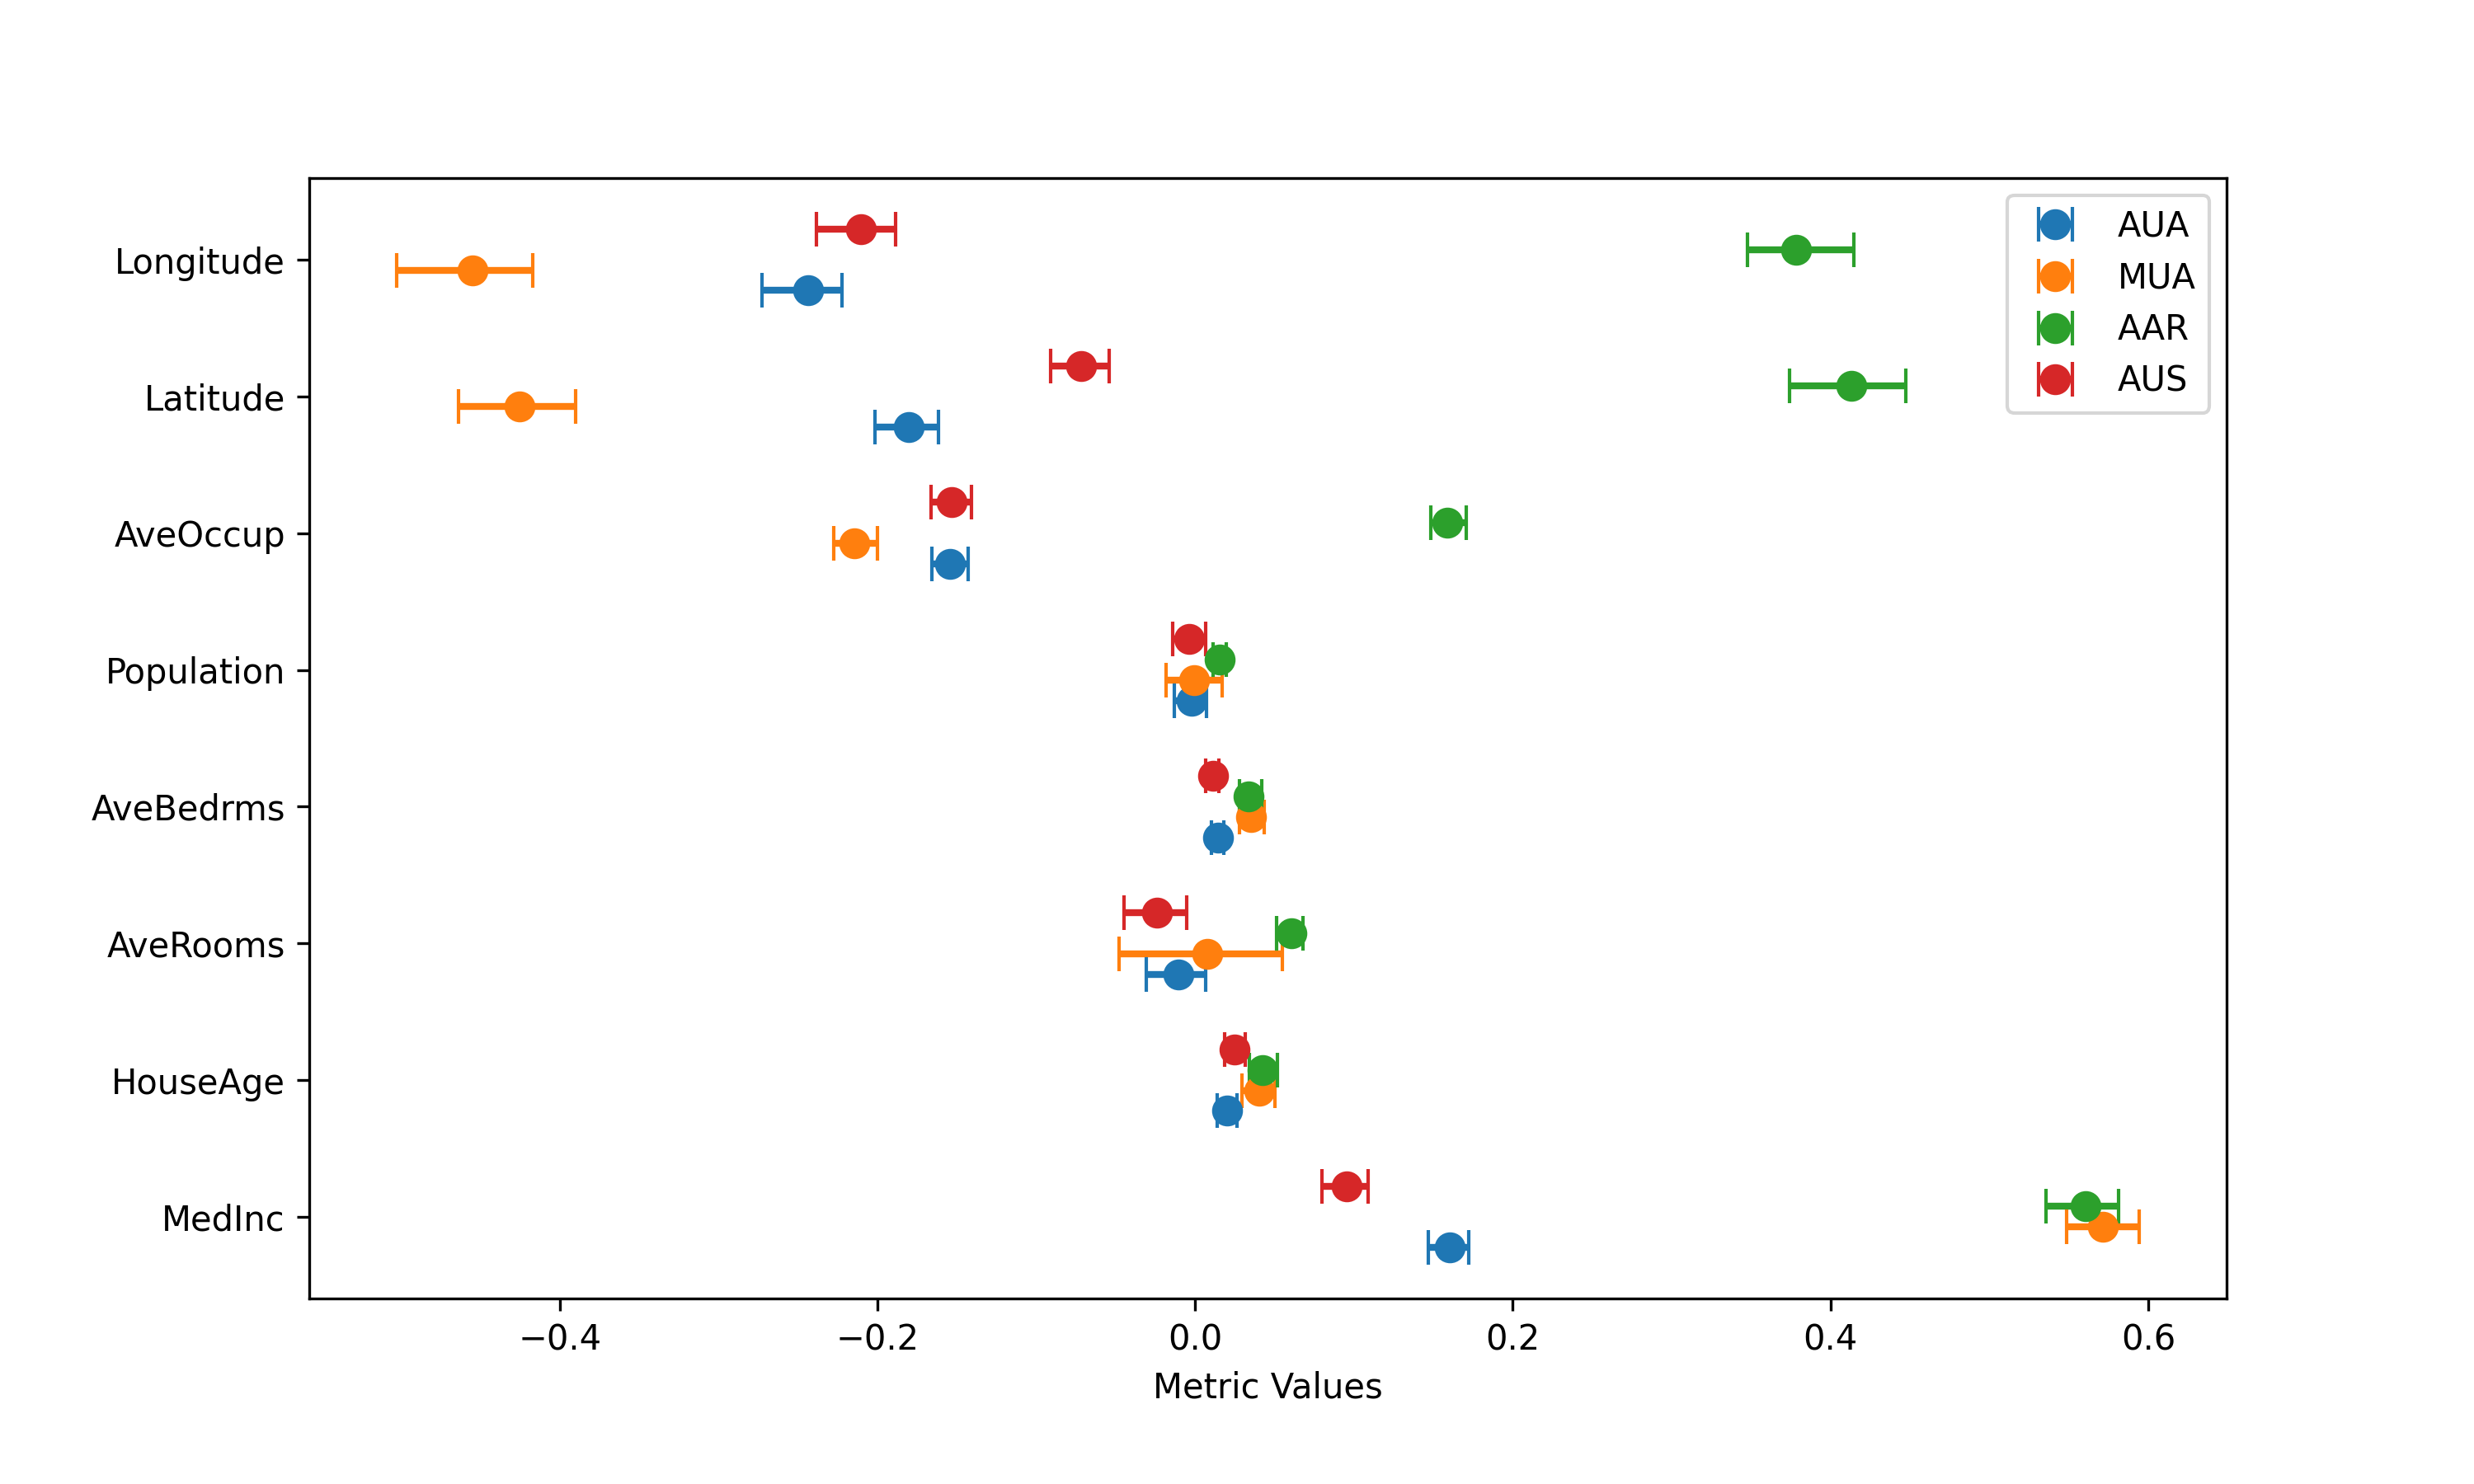
\includegraphics[width=0.98\textwidth]{images/newMetrics/housing_ale_metrics_rf_full.png}}
  \caption{Illustration of the confidence interval construction at a 5\% significance level through a data and model (full) bootstrap over 100 iterations}
    \label{fig:bootstrap_full}
\end{figure}

\begin{figure}[ht!]
\centering
  \fcolorbox{gray}{white}{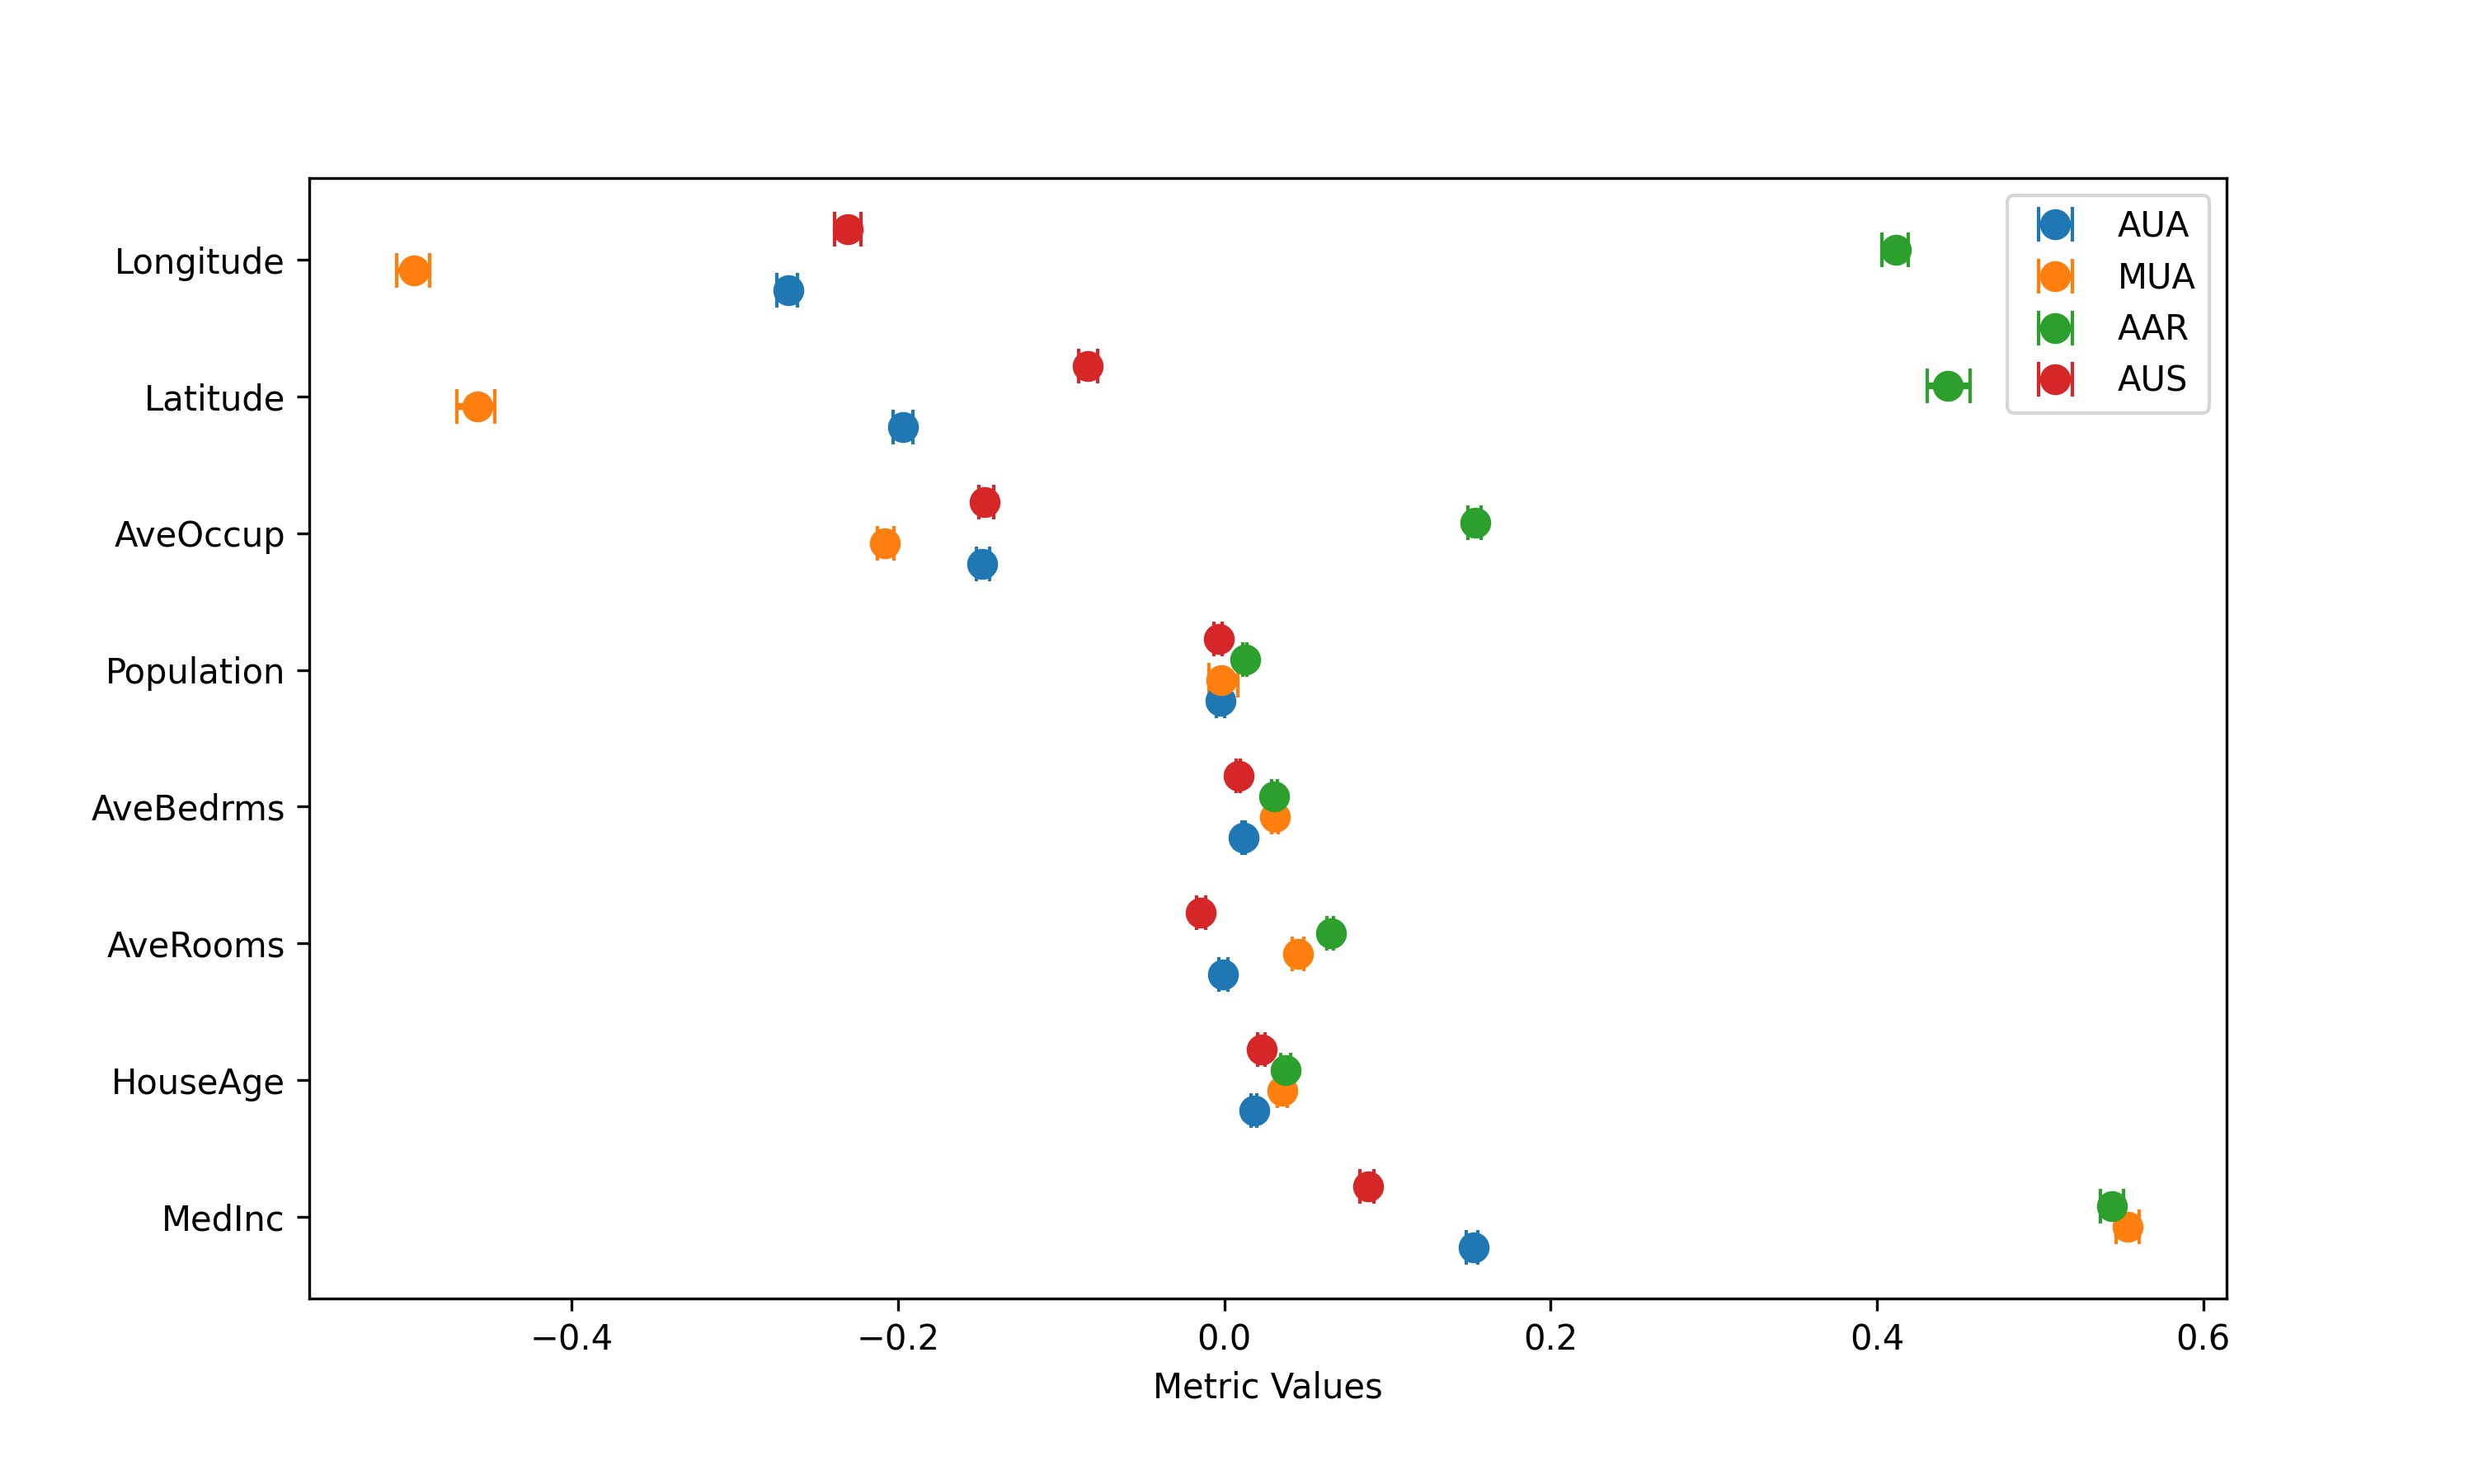
\includegraphics[width=0.98\textwidth]{images/newMetrics/housing_ale_metrics_rf_no_full.png}}
  \caption{Illustration of the confidence interval construction at a 5\% significance level through a data-only bootstrap over 100 iterations}
    \label{fig:bootstrap_no_full}
\end{figure}

\subsection{Interaction feature effects size}

Although \gls{ALE} framework can be defined for any interaction order effects \cite{Apley2020VisualizingModels}, the visualization through plots is typically reliable only up to second-order effects. This is because higher-order effects cannot be effectively represented in plots. By employing a scoring system, the interaction of n-order effects can be made more readable; however, interpretability decreases and utility becomes more limited as the value of \(n\) increases. Following \gls{ALE} definition \cite{Apley2020VisualizingModels}, the computation of scores essentially follows the algorithm \ref{algorithm:cap3}. Notably, instead of one-dimensional quantiles, n-effects analysis requires n-dimensional partitions, and an adjustment for the right interpretation of the interaction additional effect is necessary.

For a given model function \(f\), the analysis typically begins with partitioning each feature into quantiles or intervals. In the context of second-order effects, a two-dimensional grid is created by forming the Cartesian product of the quantiles of both features \cite{Apley2020VisualizingModels}. This approach is then extended to \(n\) dimensions for higher-order effects involving more features. The essence of this analysis lies in how the model's response varies across these multidimensional partitions. 

In the end, it is necessary to subtract the main effects of both features from each partition's local effects. Thus, the interpretation of the interaction is essentially the uncentered additional effect resulting from the interaction of both features.
